\section{A matched comparison of KAHM and alternative geometries}
\label{sec:matched-geometry}

% Generated from the complete matched-geometry analysis.
\newcommand{\MatchedCandidates}{13{,}440}
\newcommand{\MatchedComparisons}{42}
\newcommand{\MatchedImproved}{28}
\newcommand{\MatchedDegraded}{14}
\newcommand{\MatchedCalComparisons}{180}
\newcommand{\MatchedCalCertified}{1}


The preceding experiments do not fully separate geometry and decoder effects:
the KAHM Frobenius-budget and rollout families lack corresponding radial basis
function (RBF) and affine-hull controls. We compare all three geometries with
identical decoder choices and validation opportunities on all seven tasks.
The protocol was specified before fitting, informed by the earlier experiments.

\subsection{Design and validation selection}

Each geometry is paired with three prediction architectures, referred to as
\emph{heads} in the tables. \emph{Block direct} predicts the requested horizons
under the sum-of-block-Frobenius-norms constraint in
\eqref{eq:training-objective}. \emph{Frobenius direct} uses a single Frobenius
norm constraint on the concatenated coefficient matrix. \emph{Rollout} fits an
affine transition between feature vectors, iterates this transition, and
decodes the resulting vector into the observed signal
(Appendix~\ref{app:protocols}). Every geometry--head pair has access to the four
retained dimensions $2,6,14,30$, both history lengths, and all four preprocessing
options from Section~\ref{sec:input-scaling}. Unlike the preceding scaling
study, this comparison varies preprocessing for KAHM, RBF, and affine-hull
features alike.

Training data, horizons, origins, regularization, geometry subsampling, and
target units follow the original configurations. Direct heads share a numerical
coefficient budget, which does not make feature maps statistically equivalent.
Rollout sensitivity budgets use the fitted transition and output decoder.
Equal feature counts need not imply equal runtime or kernel-evaluation cost.

The five fitting seeds $5701$--$5705$ generate new training, validation,
calibration, and test episodes for every synthetic task. PenDigits uses new
training-stroke subsamples and geometry-fitting randomness within the same
development and held-out writer cohorts, measuring fitting variation without
new test writers.

For each task, seed, geometry, and head, the primary analysis selects
preprocessing, history length, and retained dimension by mean validation MSE
across horizons. Ties are resolved by feature count, history length,
preprocessing order (standardization, min--max, clipped min--max, raw), and
candidate name. This gives six primary comparisons per task and seed: KAHM
against each of the two alternative geometries under each of the three heads.
The selected dimension, history, and preprocessing can differ between
geometries, but the available choices are identical.

The descriptive outcome is test MSE averaged over horizons; percentage changes
use ratios of seed-averaged MSEs, not means of seed-specific percentages. Every
paired seed effect is retained; tasks are not pooled. Additional curves fix
the dimension and select history length and preprocessing by validation.
A secondary analysis also selects the head by validation; it appears in
\path{taskwise_comparisons.csv}, in rows marked
\texttt{analysis=head\_selected} and \texttt{horizon=all};
Appendix~\ref{app:matched-geometry} gives the analysis directory.

PenDigits selects each coordinate's predictor separately and weights validation
writers equally. After selection, coordinate losses and horizon losses are
averaged within each held-out writer, and the 13 writers receive equal weight.
Repeated fitting seeds do not provide additional independent writers.

\subsection{Confidence accounting and interpretation}

For each synthetic task and seed, each arm receives failure budget $0.01$:
the inherited $80/20$ allocation assigns $0.008$ to fixed candidate risk bounds
and $0.002$ to refinement comparisons. A union bound over four arms uses $0.04$;
the remaining $0.01$ is divided equally among the six primary geometry
comparisons.

For each primary comparison, we subtract KAHM squared loss from the
alternative's squared loss and average the difference over horizons within
each independent calibration episode. The resulting episode averages lie in
$[-4,4]$. Applying the paired empirical Bernstein bound
\eqref{eq:paired-improvement}, with range length $8$ and failure probability
$0.01/6$, gives a lower confidence bound on the alternative's risk minus KAHM's
risk. A positive lower endpoint certifies lower risk for that fitted KAHM
predictor. All validation selection occurs before calibration and uses
independent development data.

This allocation gives a simultaneous $95\%$ event within each synthetic
task--seed combination, not across tasks, seeds, or earlier campaigns.
Fixed-dimension and head-selected comparisons remain descriptive; an
inconclusive improvement certificate does not establish equal risks.

PenDigits retains nominal writer-level upper endpoints with failure budget
$0.0125$ per
preprocessing arm, allocated jointly over candidates, coordinates, fitting
seeds, and horizons. The allocations sum to
$0.05$. A joint confidence interpretation requires both independent and
identically distributed writers and candidate specification independent of
the writer losses used for calibration. The first assumption remains unverified;
the second is not established for this follow-up because the design was
informed by earlier results on the same cohort. Consequently, these endpoints
do not provide a new confirmatory population guarantee. No additional
independent writer cohort is available for the geometry comparisons, and
paired writer differences remain descriptive.

\subsection{Geometry, prediction architecture, and task interact}

\begin{table}[t]
\centering
\small
\setlength{\tabcolsep}{3.5pt}
\begin{tabular}{lrrrrrr}
\toprule
& \multicolumn{2}{c}{Block direct} & \multicolumn{2}{c}{Frobenius direct} & \multicolumn{2}{c}{Rollout} \\
\cmidrule(lr){2-3}\cmidrule(lr){4-5}\cmidrule(lr){6-7}
Task & RBF & Affine & RBF & Affine & RBF & Affine \\
\midrule
Harmonic & $-2.4$ (5) & $-5.1$ (5) & $-1.5$ (5) & $+6.1$ (0) & $-0.2$ (3) & $+1.2$ (1) \\
Quasiperiodic & $-2.0$ (2) & $-1.4$ (2) & $-1.7$ (3) & $+30.1$ (0) & $-6.1$ (2) & $+3.3$ (1) \\
Nonlinear AR & $-2.7$ (5) & $-4.4$ (5) & $-2.7$ (5) & $-4.4$ (5) & $-5.0$ (5) & $-4.9$ (5) \\
Logistic & $-1.0$ (3) & $-4.5$ (5) & $-0.4$ (2) & $-5.8$ (5) & $+1.7$ (1) & $-5.7$ (5) \\
Van der Pol & $-14.4$ (5) & $+9.5$ (2) & $-14.5$ (3) & $+102.7$ (0) & $-17.1$ (4) & $+92.8$ (0) \\
Duffing & $+3.8$ (3) & $+13.1$ (1) & $+10.4$ (0) & $+70.6$ (0) & $+1.4$ (3) & $+79.9$ (0) \\
PenDigits & $-15.6$ (5) & $-12.7$ (4) & $-17.2$ (5) & $-1.9$ (4) & $-17.9$ (5) & $-1.4$ (3) \\
\bottomrule
\end{tabular}
\caption{Matched geometry follow-up: percentage change in test MSE of KAHM relative to the indicated alternative, within each head. Negative values favor KAHM. Parentheses give the number of 5 fitting seeds with lower KAHM MSE. Preprocessing, history and retained dimension are selected separately for each geometry and head by validation MSE only. Percentages use ratios of MSE averaged over horizons and fitting seeds within each task; PenDigits first pools coordinate losses and equally weights eligible writers. Synthetic calibration comparisons use new episodes and a separate multiplicity allocation. The PenDigits comparisons reuse the same cohort. All test effects in this table are descriptive.}
\label{tab:matched-geometry-primary}
\end{table}


All scheduled fits completed, yielding \MatchedCandidates\ retained candidates.
Table~\ref{tab:matched-geometry-primary} reports all \MatchedComparisons\ primary
task--head--alternative contrasts: KAHM has lower mean test MSE in
\MatchedImproved\ and higher mean test MSE in \MatchedDegraded. These contrasts
share tasks and fitted models; they are not independent evidence for a
universally preferred geometry. Table~\ref{tab:matched-geometry-mse} gives
absolute errors for all nine geometry--head families.

On nonlinear AR, KAHM improves on both geometric alternatives under every head
in all five fitting seeds. Its block-direct mean MSE is $0.00456$, compared
with $0.00511$ for ridge AR and $0.00523$ for quadratic regression. On PenDigits,
the KAHM reductions relative to RBF are $15.6\%$, $17.2\%$, and $17.9\%$ for
block direct, Frobenius direct, and rollout, respectively, with lower loss in
all five seeds. The corresponding mean reductions relative to affine-hull
features are $12.7\%$, $1.9\%$, and $1.4\%$, with four, four, and three favorable
seeds. This advantage is specific to the geometric comparison. PenDigits
Frobenius-direct KAHM MSE is $0.00504$, while ridge AR and quadratic regression
achieve smaller MSEs of $0.00184$ and $0.00102$.

The oscillator controls limit how much of an accuracy gain can be attributed
to KAHM geometry. On Van der Pol, KAHM mean MSE is $14.4$--$17.1\%$ lower than
RBF across the three heads, yet exceeds affine-hull MSE by $9.5\%$, $102.7\%$,
and $92.8\%$, respectively. On Duffing, the corresponding excesses over
affine-hull MSE are $13.1\%$, $70.6\%$, and $79.9\%$. The affine-hull advantage
under Frobenius-direct and rollout heads occurs in every fitting seed on both
oscillators. A gain from changing a KAHM decoder or its preprocessing therefore
does not by itself establish a benefit of KAHM geometry. Mean effects can also
disagree with most seed-specific effects: the favorable quasiperiodic
block-direct means against both alternatives occur with lower KAHM loss in
only two of five seeds.

\begin{figure}[p]
\centering
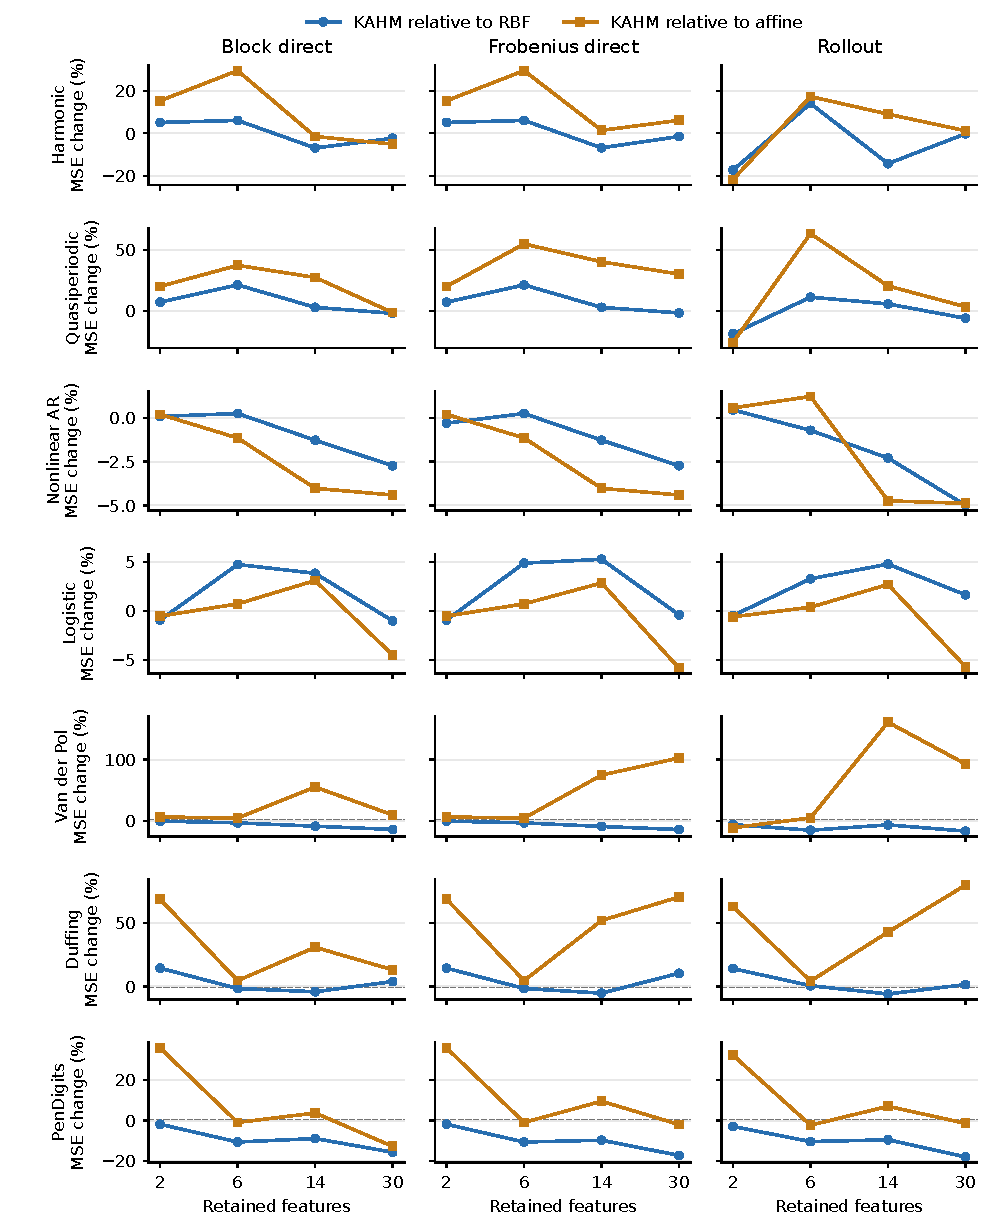
\includegraphics[width=\linewidth]{figures/matched_geometry_dimensions.pdf}
\caption{Percentage change in mean all-horizon test MSE at each fixed retained
dimension: $100(\mathrm{MSE}_{\rm KAHM}/\mathrm{MSE}_{\rm alternative}-1)$,
where each MSE is averaged over five fitting seeds. Negative values favor
KAHM. History length and preprocessing are selected by validation at each
point. PenDigits first averages coordinate losses and weights writers equally.}
\label{fig:matched-geometry-dimensions}
\end{figure}

Figure~\ref{fig:matched-geometry-dimensions} reports every fixed-dimension
comparison. On PenDigits, KAHM has lower mean MSE than RBF at all four
dimensions under each head, so the advantage cannot be explained solely by a
larger selected feature count. Its ranking against affine-hull features changes
with dimension. On nonlinear AR, all three KAHM heads improve on both
alternatives at dimensions 14 and 30, while the smaller dictionaries have
mixed effects. Theorem~\ref{thm:replication-invariance} concerns population
optima for fixed retained blocks. These curves also reselect history length and
preprocessing at each dimension and therefore do not test that theorem.

Only \MatchedCalCertified\ of the \MatchedCalComparisons\ planned synthetic
calibration comparisons has a positive improvement lower endpoint: Van der
Pol, seed 5703, KAHM rollout versus RBF rollout, with a lower bound of
$0.00107$ on the all-horizon MSE reduction. The other 179 comparisons remain
inconclusive. This positive statement concerns those two fitted predictors
within the declared simultaneous event for that repetition. It is distinct
from the descriptive test-effect table and gives no population comparison
for PenDigits.
